% !TEX root = ../thesis.tex

\chapter{AVPipe的测试与评估}

在这一章中,我们将展示由AVPipe构建的不同视频流处理任务。并通过对具体视频处理任务在不同平台的运行来展示AVPipe提供的性能优化。

\section{测试任务}
本小节会对我们所使用的视频处理任务进行简单介绍。以下模型/处理流程都是对一些出名的开源项目在AVPipe框架下的实现。
% \subsection{视频物体识别任务} % TODO

\subsection{视频人体姿态估计任务}
人体姿态估计是指识别图像中人体各个关节点的位置。我们基于Sun et al.提出的HRNet(High Resolution Network)\cite{sun2019deep}来构建本任务。HRNet是一个多层级的深度CNN模型,它主要利用了多尺度图像中的空间结构信息来提高检测精度。我们在图\ref{fig:pose_dag}已经展示了基于HRNet的人体检测估计的数据处理流程。在这一处理流程中,预处理后的图像数据会被送入HRNet进行推理,其输出是一个包含人体关键点信息的热图(heat map)张量,在后处理过程中,我们会对这个原始输出行进高斯滤波(filter),多通道峰值选择(maxPred)等操作,最终获得一个与输入图片相对应的关键点坐标列表。在进行最后的输出渲染时,我们只显示预测置信度高于于预设阈值的关键点。本任务中各个步骤之间的依赖关系较为简单,
可以将处理过程分为预处理,神经网络推理,后处理三部分进行多线程流水线优化。这也正是AVPipe自动多线程优化所得的结果(图\ref{fig:pose_dag})。方便起见,我们会在后续测试中将该视频处理任务简称为Pose。

\subsection{视频手部检测与追踪任务}
与人体姿态估计任务类似,手部检测与追逐是指检测出图像的人手,并对手部的动作进行捕捉。在这里我们采用了Google提出的手部追踪处理流程\cite{mediapipe_hand}。图\ref{fig:hand_dag}展示了该处理流程在AVPipe中的可视化。
该处理流程用到了两个CNN模型分别用来做手部检测(PalmCNN)与手部关键点定位(HandCNN)。首先经过预处理的图像数据会送入PalmCNN,PalmCNN是一个基于SSD(Single Shot MultiBox Detector)\cite{liu2016ssd}模型进行简化的检测模型,在拿到PalmCNN的原始检测结果后,需要通过尺寸缩放(decodeBoxes),非极大值抑制(NMS)等后处理操作获得可以对应原图的手部检测框。在接下来的处理流程中,手部检测结果会根据其对应的检测框进行旋转,剪裁与缩放,构成一批手部位于图像中心的图片,这批图片会在预处理后送入HandCNN进行关键点定位。最后,关键点信息会通过转换(rotateBack)对应回原图中的坐标。\par
为了减少处理过程中的冗余计算,加快流程的处理速度,该手部追踪处理流程还在其检测算法流程上进行了针对视频任务的优化。由于人手在连续视频帧中的位移量一般较小,故可以直接使用上一帧关键点检测结果估计人手在下一帧中出现的位置,从而PalmCNN不必每帧都运行,它只需要在一些关键帧或检测目标丢失时运行。为实现这部处理逻辑,我们在AVPipe中设立了两个自定义的计算模块multiplexer和streamMerger用来选择运行正确的数据源。未将本帧计算结果转播到下一帧去,我们在处理流程中加入了timeUpdate模块,其产生的数据包会被标记为下一帧的时间戳(图\ref{fig:hand_dag}中的虚线箭头),这点也会在建立计算图时由Stream进行必要的特殊初始化。\ref{fig:hand_dag}也展示了该处理任务在4个线程下的划分,该划分将两个CNN放入了两个不同的线程中,线程间不存在局部依赖,
每个线程的耗时都不超过最耗时模块的用时,满足我们对该计算图的优化期望。在测试过程中,我们会分别对使用了上述算法优化(由Hand-opt表示)和未使用上述算法优化的处理流程(由Hand-raw表示)进行性能测试。

\begin{figure}[!bt]
    \centering
    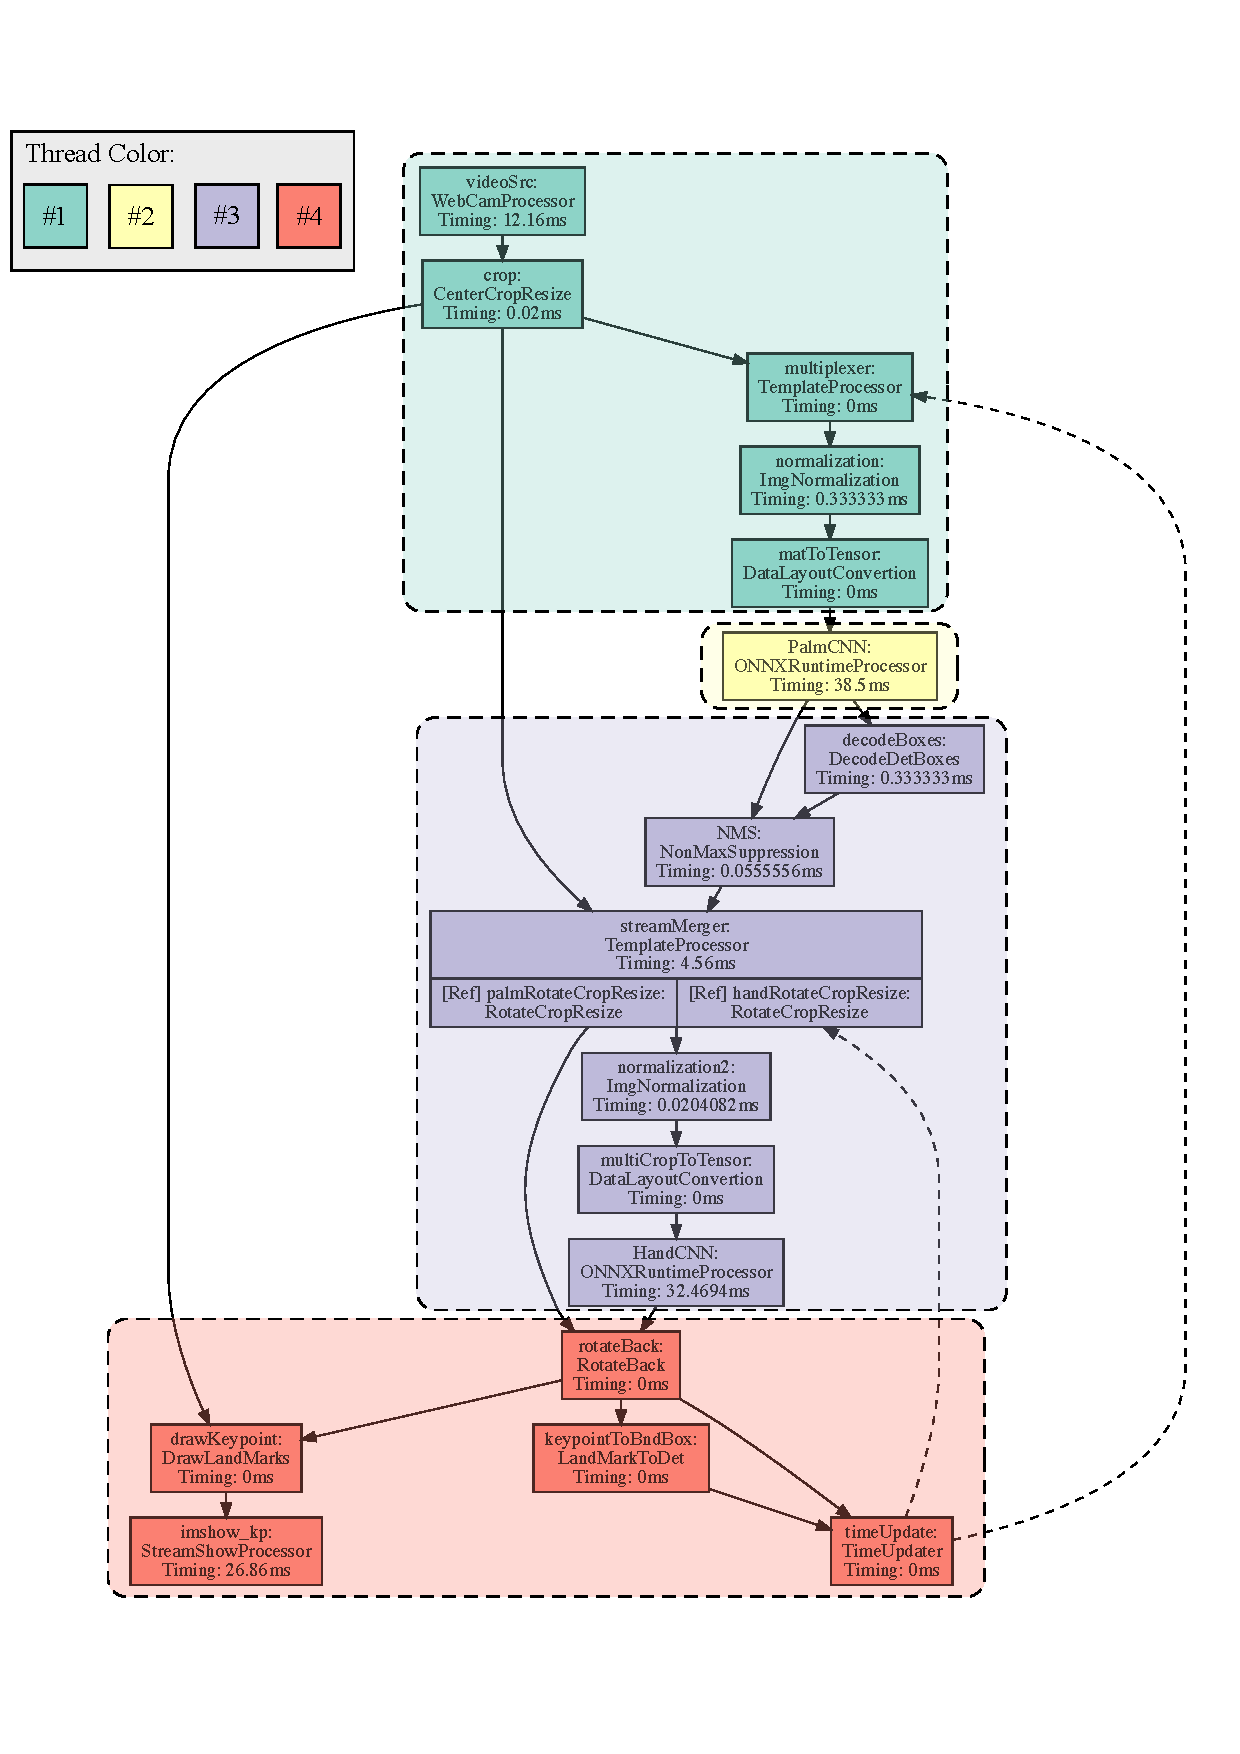
\includegraphics[width=0.7\textwidth]{figure/AVP_multi_hand_tracking.pdf}
    \caption[手部追踪任务在AVPipe框架下处理流程的可视化]{手部追踪任务在AVPipe框架下处理流程的可视化。图中虚线连接表示该模块的在本时间戳的输出会在下一时间戳中使用。 由于本图的连接较为复杂,为便于观察,我们没有提供如图\ref{fig:pose_dag}中的Stream可视化,只保留模块间连接。
    节点运行时间信息来自Intel i5-8210Y处理器的MacBook Air的预运行。}
    \label{fig:hand_dag}
\end{figure}

\section{运行环境与参数设置}
目前AVPipe框架完成了对macOS,Linux以及Windows这三大桌面操作系统的支持\footnote{我们会在以后尽可能地提供对移动平台的支持,但这部分并不属于本研究课题所关注的重点。}。同时,由于AVPipe框架的目标设备主要是用户个人的终端,而非高性能的服务器,因此我们选择的macOS和Windows这两个主流平台下的便携笔记本电脑作为测试设备(我们手上持有的计算设备也只能支持我们选择这样的测试设备)。对macOS平台,我们使用了一台MacBook Air,其搭载了
Intel i5-8210Y双核处理器;对Windows平台,我们使用了一台ThinkPad X1 Carbon,其搭载了Intel i5 10210u四核处理器。更多核心数量能为多线程运行带来更好的性能,这一点我们也可通过对比这两款设备的处理速度来进行观察。
为体现AVPipe在多硬件场景下的支持,我们还在后续测试中使用了Intel Neural Compute Stick 2\footnote{\url{https://software.intel.com/content/www/us/en/develop/hardware/neural-compute-stick.html}}这一神经网络加速器,以及Intel的核心显卡进行处理流程的构建。\par

在测试过程中,为了尽可能减少其他因素对运行结果的影响,同一处理任务在不同平台下均使用同一视频文件的前200帧作为输入进行分析。在运行视频处理任务时,我们会尽可能关闭系统中其他正在运行的高资源占用进程。


\section{性能对比分析}

\section{多线程优化验证}

\section{本章小结}

